\documentclass[../master]{subfiles}
\begin{document}
\chapter{テスト実験に向けて}
\label{chap::experiment}
\section{大阪大学14 MeV 中性子工学実験装置 (OKTAVIAN)}
大阪大学工学研究科のOKTAVIAN~\cite{oktavian} ではDT 反応により\SI{14}{\mega\electronvolt}の中性子を発生させることができる.
図\ref{pic::oktavian-sketch}にOKTAVIAN の施設図を示す.
OKTAVIAN は1981年から運転を開始し,核融合中性子工学研究に用いられてきた.
コッククロフト・ワルトン型加速器を用いて加速したデューテリウムをトリチウムターゲットに照射することで,
\SI{14}{\mega\electronvolt} の中性子を生成する.
OKTAVIAN にはパルスビームラインとDCビームラインの2つのビームラインがある.
パルスビームラインは大実験室に設置されたトリチウムターゲットを用いて,
DC ビームラインは重照射室に設置されたトリチウムターゲットを用いて中性子を生成する.

DC ビームラインで生成された中性子はトリチウムターゲットを中心に放射状に重照射室へ放出される.
図\ref{pic::hole}に示すように,この中性子を大実験室側へ取り出すための半径約\SI{55}{\milli\metre}の取り出し穴が
重照射室と大実験室を隔てる壁に設けられている.
図\ref{pic::hole}は重照射室と大実験室を隔てる壁を大実験室から撮影した写真である.
この取り出し穴から中性子を取り出すことで,
半径約\SI{55}{\milli\metre}にコリメートされたDC 中性子ビームを得ることができる.
ただし,DC ビームであるため中性子が入射した時間情報を得ることはできない.
一方で,パルスビームラインでは図\ref{pic::pulse_beam_line}のように大実験室中にトリチウム標的が設置されているため,
中性子をコリメートすることができない.
また,大実験室に測定装置を置いた場合,
壁などから反跳した中性子がバックグラウンドとなってしまう.
その反面,パルス状に中性子が発生するので,中性子の時間情報を得ることができる.
本測定では,バックグラウンドイベントを低減することや,
中性子の入射領域を制限できることから,DC ビームラインを用いて測定を行う予定である.
また,取り出し穴に任意の形状のコリメータを入れることで,
ビームの形状を制御することができる.
\begin{figure}
  \centering
  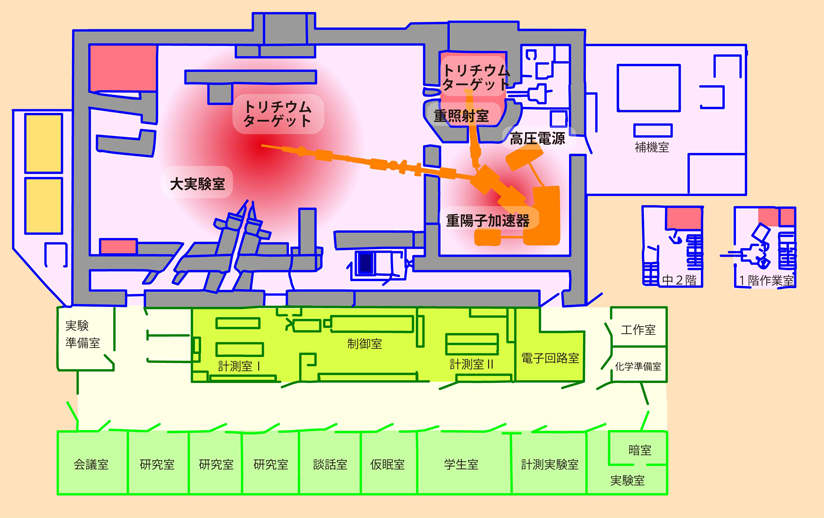
\includegraphics[clip, width=0.9\columnwidth]{oktavian-sketch.png}
  \caption[OKTAVIAN の施設図.]
          {OKTAVIAN の施設図~\cite{oktavian}.パルスビームラインとDC ビームラインがそれぞれ大実験室と重照射室に伸びている.}
  \label{pic::oktavian-sketch}
\end{figure}
\begin{figure}[h]
  \centering
  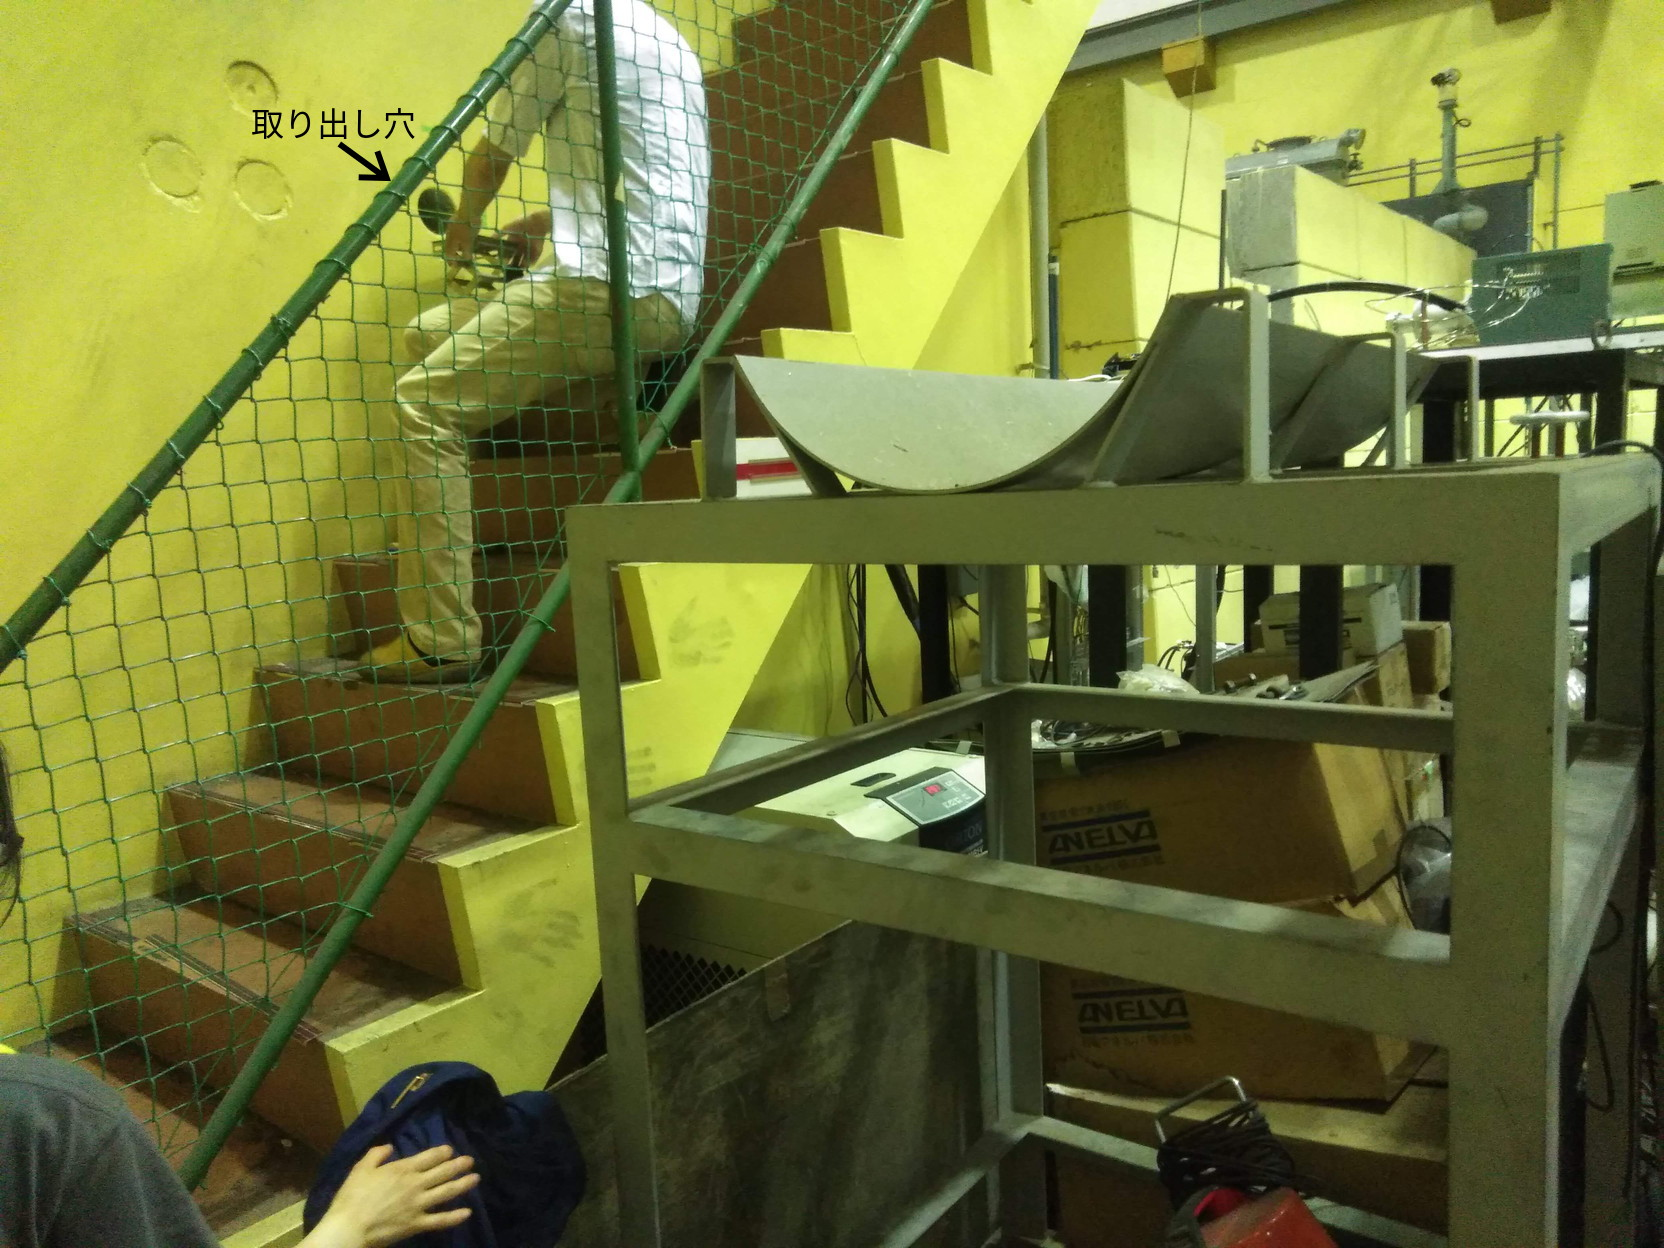
\includegraphics[clip, width=0.9\columnwidth]{IMG_20190805_152904_drawed.jpg}
  \caption{大実験室側からDC中性子の取り出し穴のある壁を見たときの様子.}
  \label{pic::hole}
\end{figure}
\begin{figure}[h]
  \centering
  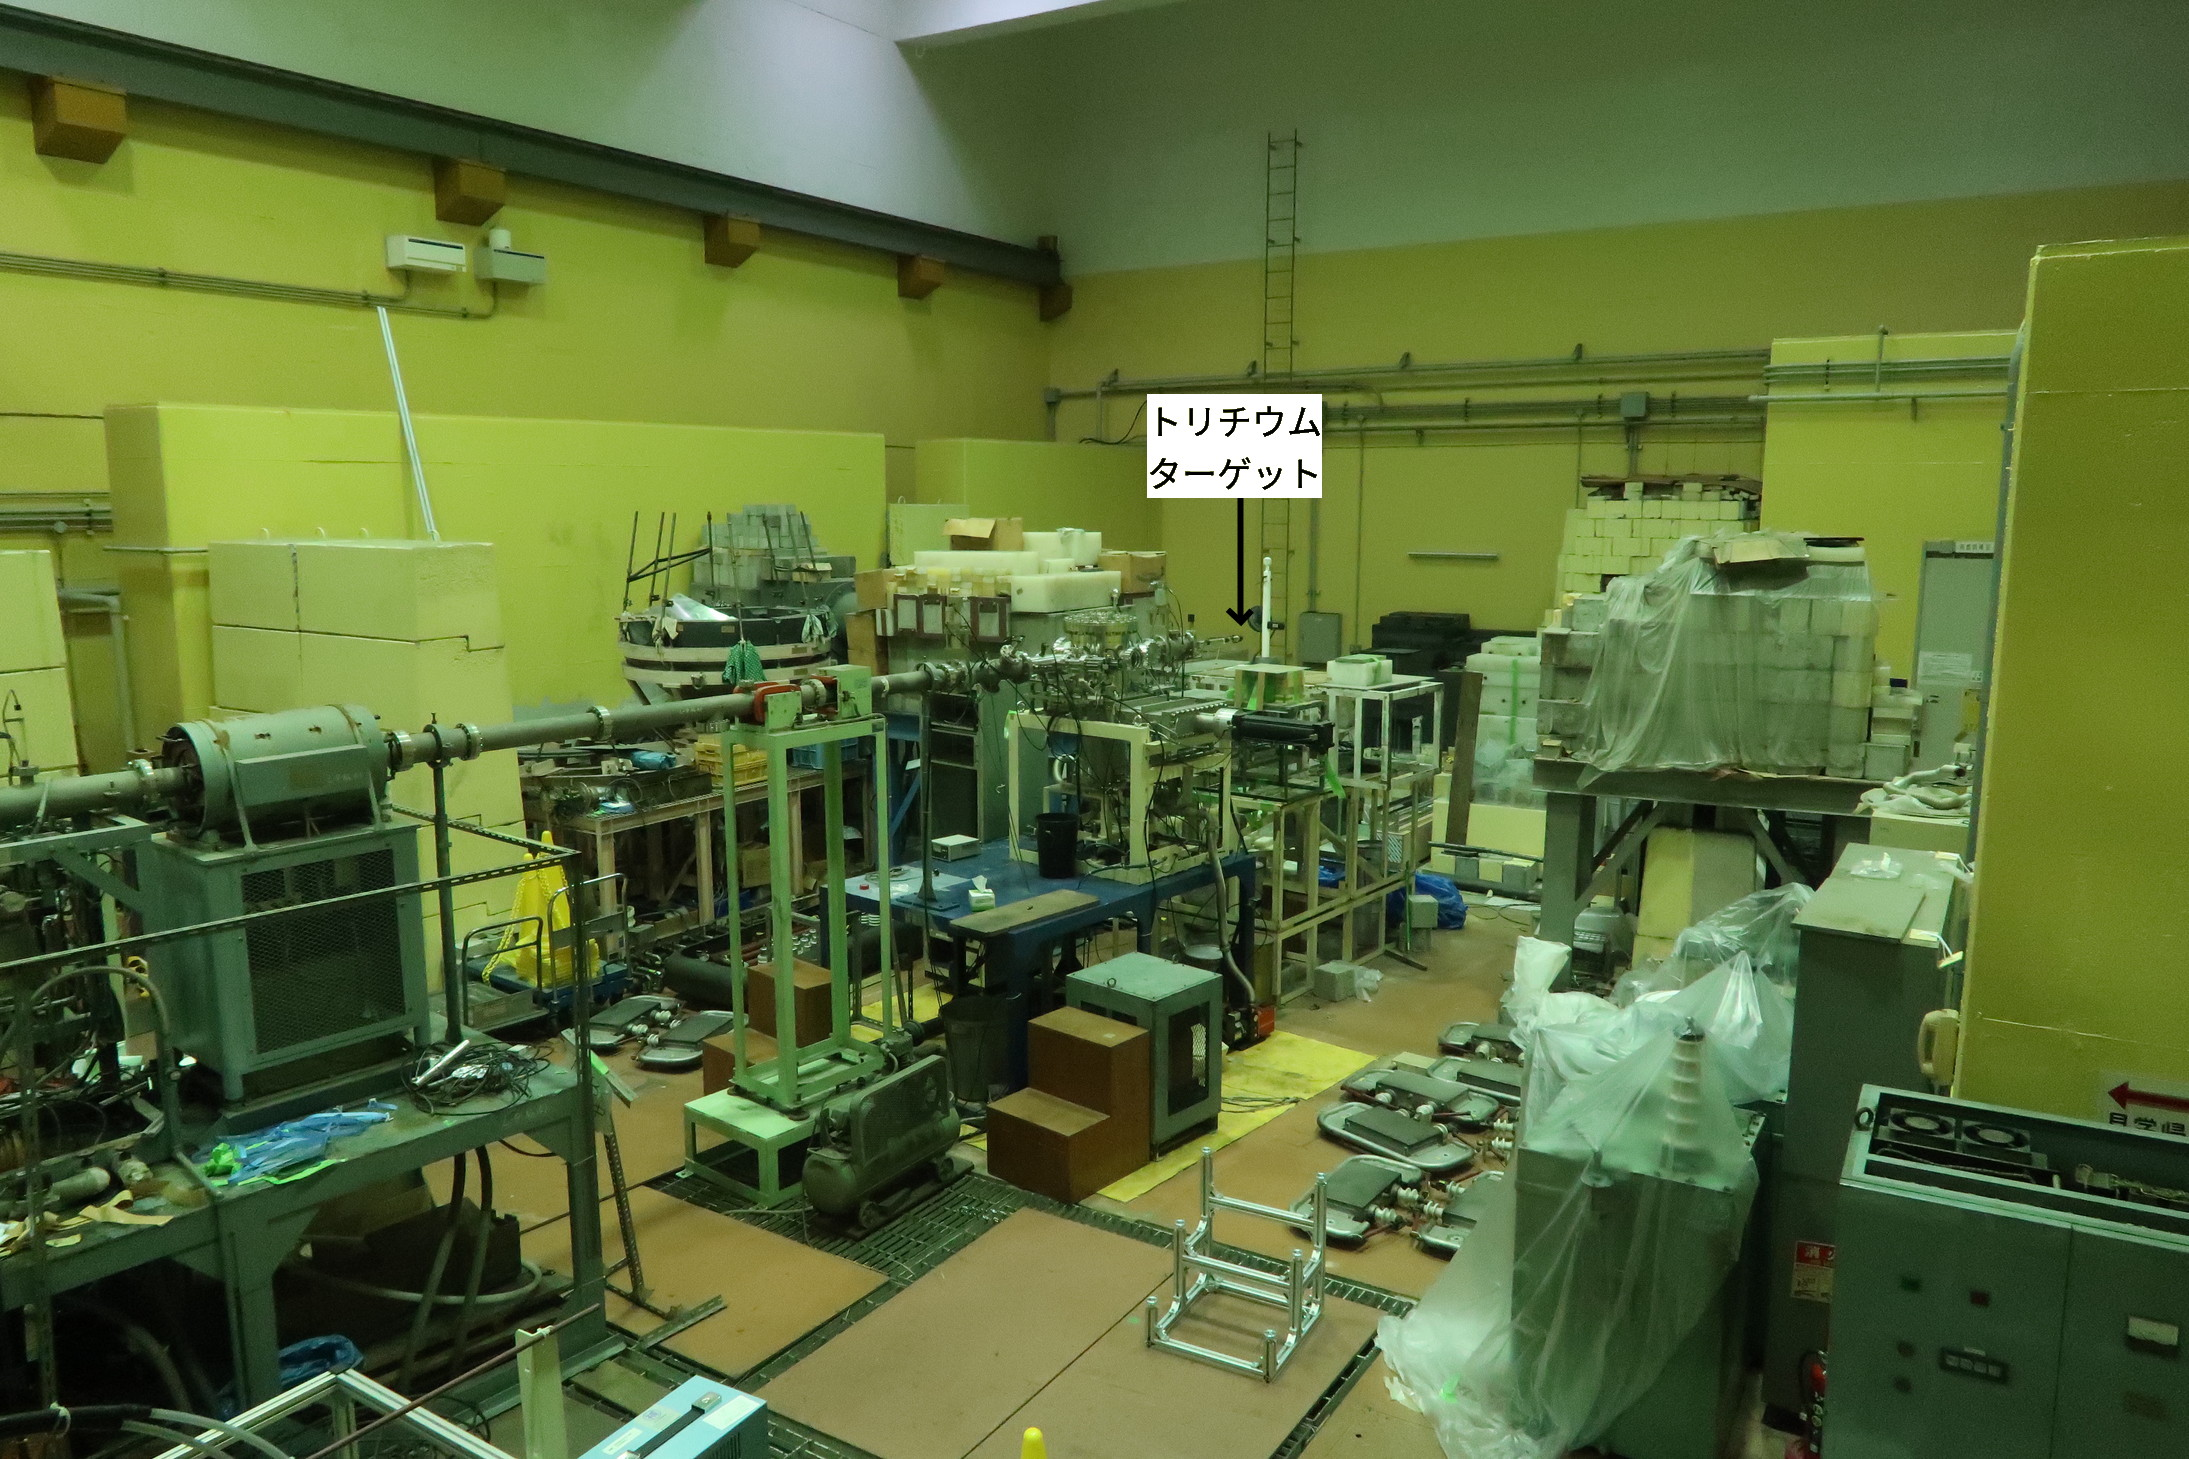
\includegraphics[clip, width=0.9\columnwidth]{IMG_2778_drawed.jpg}
  \caption[大実験室およびパルスビームライン.]
          {大実験室およびパルスビームライン.
            写真中央にパルスビームラインのトリチウムターゲットが設置されている.
          写真右手前から加速されたデューテリウムが照射される.}
  \label{pic::pulse_beam_line}
\end{figure}
%\begin{figure}
%  \centering
%  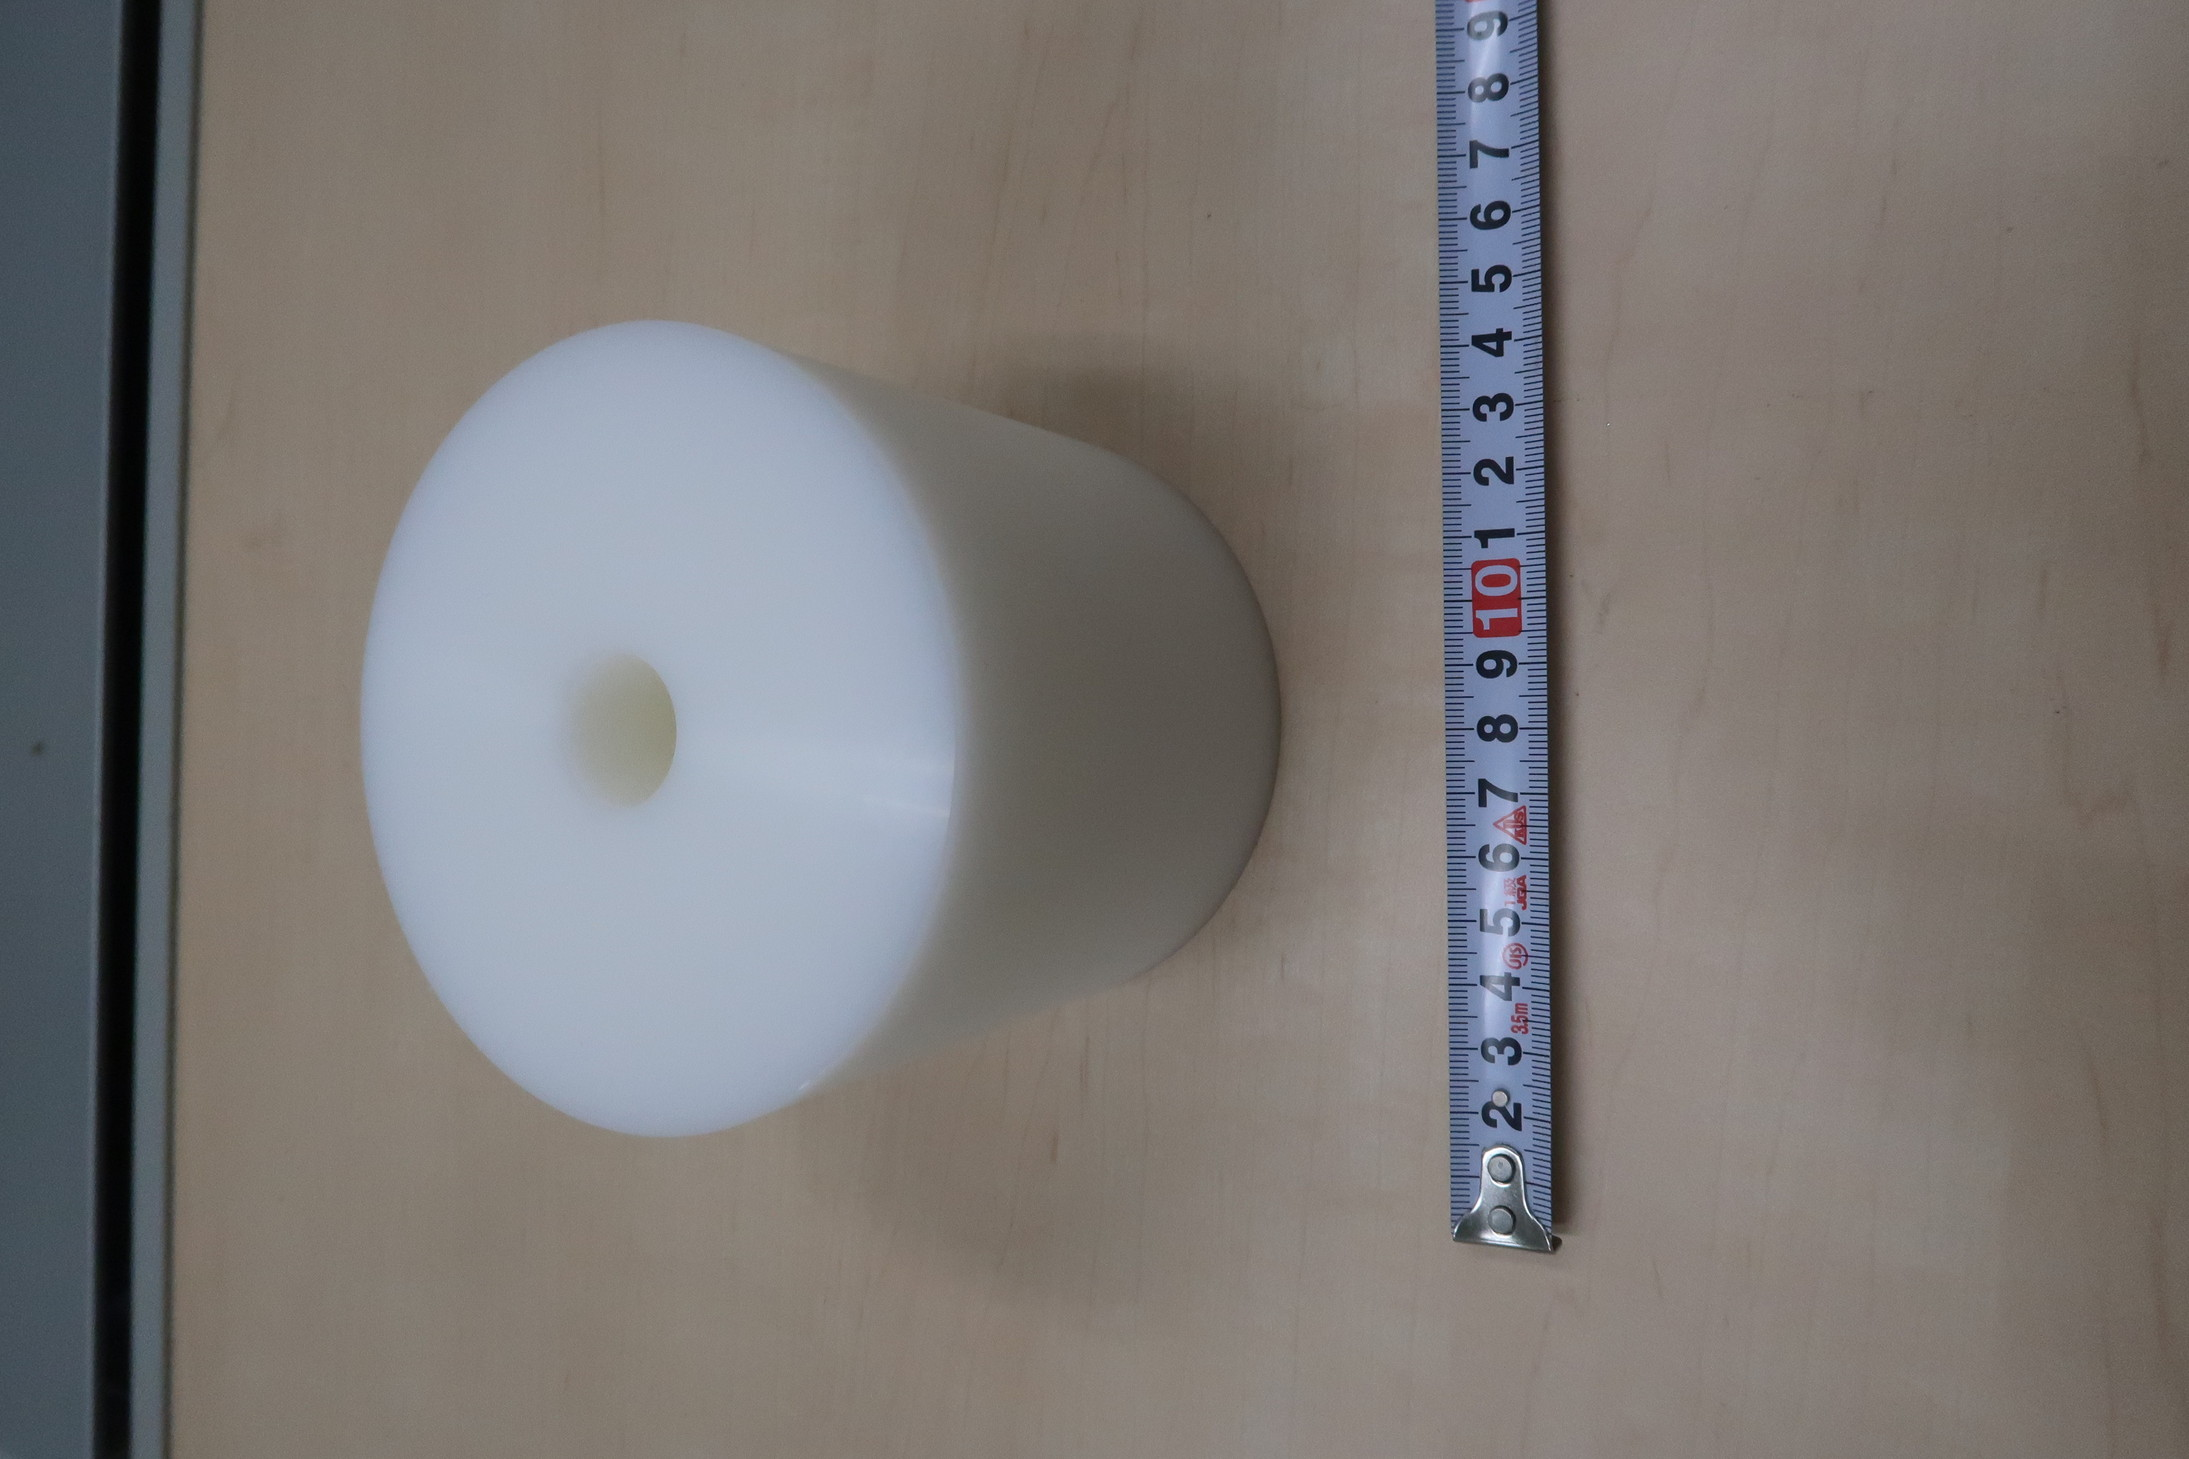
\includegraphics[clip, width=0.8\columnwidth, angle=270]{IMG_2755.jpg}
%  \caption{コリメータ.外半径\SI{53}{\milli\metre},内半径\SI{10}{\milli\metre}の円柱型のポリエチレンを用いる.}
%  \label{pic::neutron_collimator}
%\end{figure}

\section{中性子ビーム}
\subsection{ビームサイズを制限する必要性}
中性子ビームは可能な限り空間的な広がりが小さいことが望ましい.
例えば,半径\SI{50}{\milli\metre}の広がりを持つ中性子ビームを用いると,
散乱点が$y$軸方向に\SI{100}{\milli\metre}の広がりを持つ.
%gridの座標を$y = \SI{0}{\milli\metre}$,plateの座標を$y = \SI{140}{\milli\metre}$とし,
%ビームの中心が$y = \SI{70}{\milli\metre}$の位置にあるとすると,
%中性子ビームは$y = $\SIrange{20}{120}{\milli\metre}の範囲に入射する.
%$y = \SI{120}{\milli\metre}$の位置で散乱が起きると,
%有感領域はgrid方向に\SI{120}{\milli\metre},plate方向に\SI{20}{\milli\metre}となる.
%反対に,$y = \SI{20}{\milli\metre}$の位置で散乱が起きると,
%有感領域はgrid方向に\SI{20}{\milli\metre},plate方向に\SI{120}{\milli\metre}となる.
しかし,MAIKo TPC はトラックの周囲に発生した電子が読み出し面に到達する時間差を用いて$y$座標を検出しているため,
絶対値を決定できない.
すると,図\ref{fig::sensitive_area}のように,ビーム入射範囲のどこで散乱が起きたのか判別できない.
%$y = \SI{120}{\milli\metre}$と$y = \SI{20}{\milli\metre}$のどちらで散乱が起きたのかを区別できない.
図\ref{fig::sensitive_area}の例では,取得されたデータが同じであっても上の場合はトラックが有感領域から出てしまっている.
トラックの長さと方向から$\alpha$粒子のエネルギーと運動量を決定するには,
トラックが有感領域中で停止しなければならない.
どちらの場合でも確実に有感領域中で停止したと保証するためには,
有感領域の$y$軸方向の長さからビームの$y$軸方向の広がりを引いた領域しか用いることができない.
半径\SI{50}{\milli\metre}のビームを用いると,
散乱点から$y$軸方向に\SI{\pm20}{\milli\metre}を実質の有感領域としなければならない.
実質の有感領域が小さいと領域外に出ていく$\alpha$粒子の数が増えてしまい,
解析に使えるイベントの割合(検出効率)が減少してしまう.
そのため,中性子ビームの$y$軸方向のサイズは可能な限り小さいのもが望ましい.
その反面,ビームを細くすると
%標的で生成された中性子を制限することになるので,
中性子のビーム量が低下してしまう.
%この2つの効果を考慮して収量が大きくなるビームサイズを決定する.
\begin{figure}
  \centering
  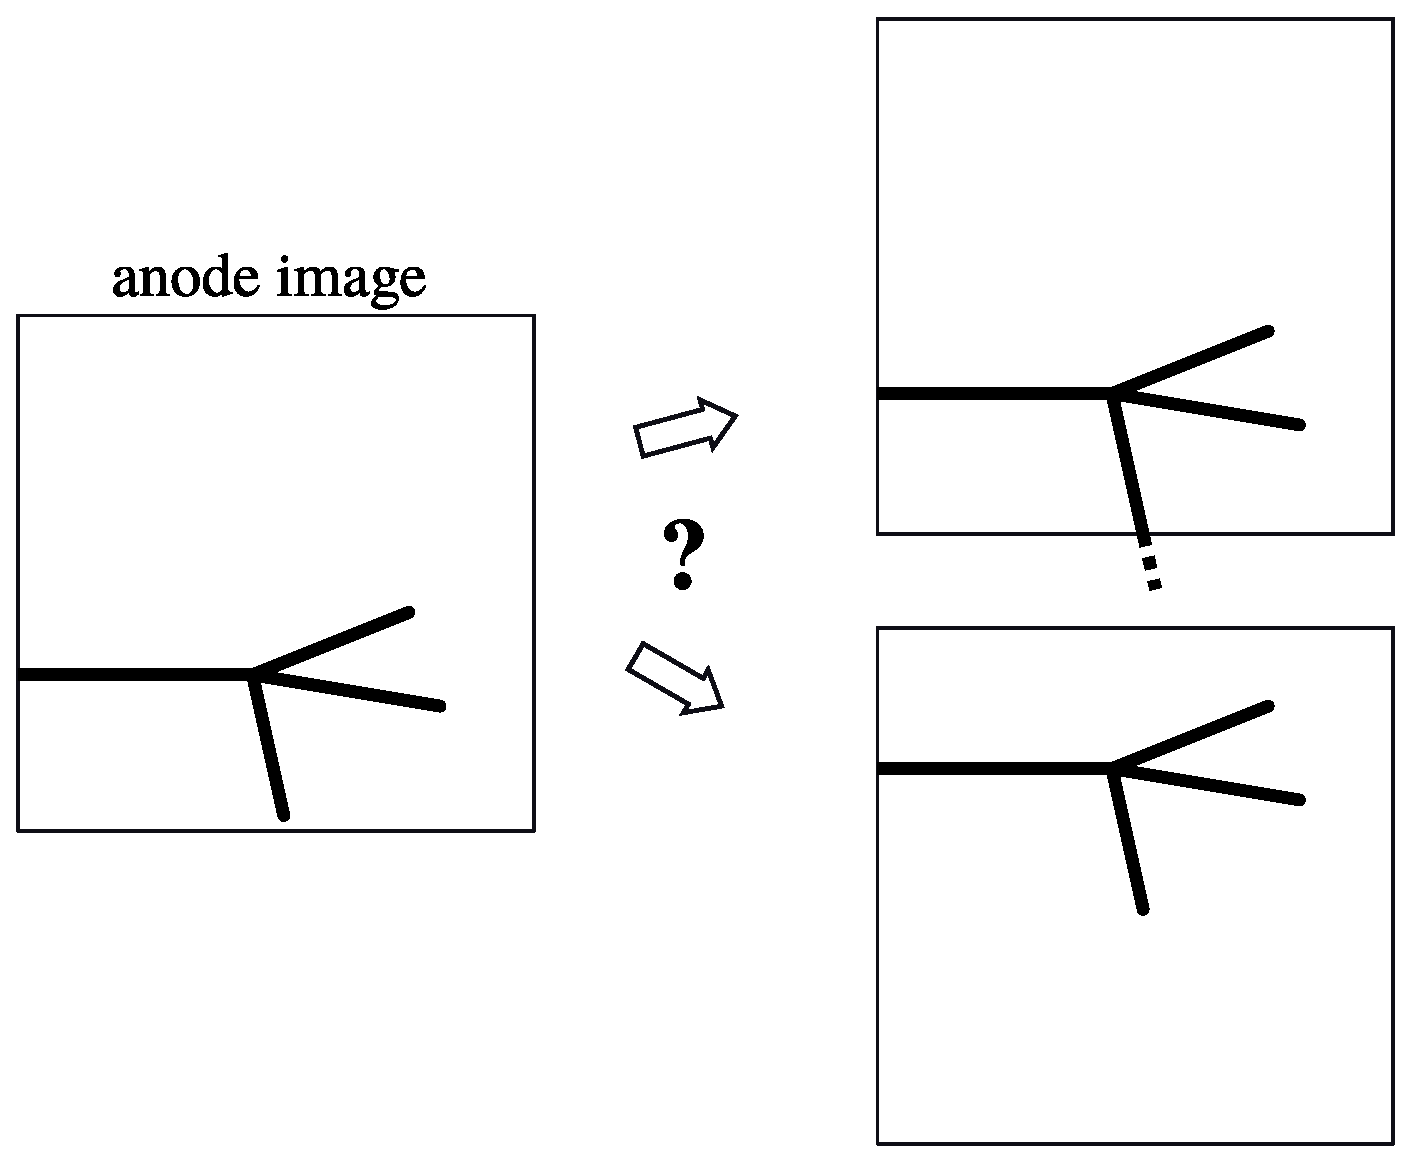
\includegraphics[clip, width=0.7\columnwidth]{sensitive_area.eps}
  \caption[ビームサイズが大きいときの散乱事象.]
          {ビームサイズが大きいときの散乱事象.
            右上のように領域外にトラックが出ているのか,右下のように領域内で停止したのか区別ができない.}
  \label{fig::sensitive_area}
\end{figure}

\subsection{立体角と検出効率によるビームサイズの決定}
重照射室内のトリチウムターゲットから中性子が$4\pi$に等方的に放出していると仮定すると,
中性子の収量はコリメータの立体角で決定される.
重照射室の模式図を図\ref{fig::jushosha_room}に示す.
トリチウムターゲットから重照射室の大実験室側の壁までの距離は\SI{1.46e3}{\milli\metre},
壁の厚さは\SI{1.00e3}{\milli\metre}である.
この壁に半径\SI{55}{\milli\metre}の穴が設けられており,そこから大実験室側へ中性子を取り出す.
この壁の穴にコリメータを設置することで任意の形に中性子ビームの形状を設定できる.
ここでは,円柱の中央に半径$r$~\si{\milli\metre}の穴が開いたコリメータを考える.
すると,立体角は$\pi\times r^2/\left(2.46\times10^3\right)^2$となる.
\begin{figure}
  \centering
  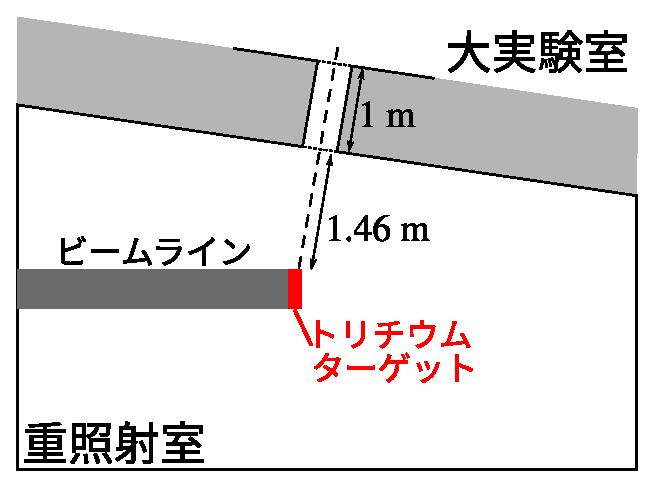
\includegraphics[clip, width=0.65\columnwidth]{jushosha_room.eps}
  \caption{重照射室の模式図.トリチウムターゲットから大実験室まで\SI{2.46}{\metre}である.}
  \label{fig::jushosha_room}
\end{figure}

%MAIKo TPC ではトラックの長さと方向からエネルギーと運動量を決定するため,
%トラック全体を正しく抽出することが必要となり,MAIKo TPC の有感領域内で停止しない$\alpha$粒子は解析に用いることができない.
%ここで,MAIKo TPC の有感領域中で全ての$\alpha$粒子が停止する割合を検出効率とする.
%検出効率が大きくなるような実験条件が望ましい.
図\ref{fig::alpha_E_dist}のエネルギー分布,ビームの通る円柱内で一様な散乱点を仮定して,
$\alpha$粒子の検出効率を求めた.
半径\SIrange{1}{50}{\milli\metre}でのコリメータの立体角の割合と検出効率を
表\ref{tab::solid_angle_percent}に示す.
検出効率は\SI{10}{\milli\metre}以下ではほとんど変化がない.
\SIlist{1;5;10}{\milli\metre}を比較すると,
立体角は\SI{10}{\milli\metre}が最も大きい.
大きな検出効率を持ちつつ,立体角が大きい\SI{10}{\milli\metre}のコリメータを用いる.
%コリメータの立体角と検出効率の積が最も大きくなるところが収量が最も大きくなる.
\begin{table}
  \centering
  \caption{コリメータの半径とコリメータの立体角,検出効率.}
  \label{tab::solid_angle_percent}
  \begin{tabular}{ccc}
    \toprule
    コリメータの半径 (\si{\milli\metre}) & 立体角 (\si{\steradian}) & 検出効率 (\si{\percent})\\% & 積\\
    \midrule
     1 & $5.19\times10^{-7}$ & 48.9 \\
     5 & $1.30\times10^{-5}$ & 48.7 \\%& $6.33\times10^{-6}$ \\
    10 & $5.19\times10^{-5}$ & 48.2 \\%& $2.50\times10^{-5}$ \\
    20 & $2.08\times10^{-4}$ & 46.6 \\%& $9.69\times10^{-5}$ \\
    30 & $4.67\times10^{-4}$ & 39.2 \\%& $1.83\times10^{-4}$ \\
    40 & $8.31\times10^{-4}$ & 26.3 \\%& $2.19\times10^{-4}$ \\
    50 & $1.30\times10^{-3}$ & 10.3 \\%& $1.34\times10^{-4}$ \\
    \bottomrule
  \end{tabular}
\end{table}

\subsection{コリメータの材質}
中性子を遮蔽する物質として,陽子を多く含むポリエチレンや吸収断面積が大きいホウ素が広く用いられている.
ポリエチレンとホウ素入りポリエチレンでの中性子の遮蔽度合いをPHITS (Particle and Heavy Ion Transport code System)
ver.~3.14~\cite{phits}を用いて計算した.
PHITS は原子力機構が中心となって開発を行っている物質中での放射線の挙動をシミュレートするモンテカルロ計算コードである.
PHITS の入力ファイルを付録\ref{chap::phits-input}に示す.
図\ref{collimator_xy_pos}は中性子がコリメータを通過したときの位置分布である.
%ポリエチレンとホウ素入りポリエチレンの両方共,半径\SI{10}{\milli\metre}のみ多くの中性子が通過していることが分かる.
%また,遮蔽されている部分は中心と比較して1桁以上中性子の量が少ないことが分かる.
%2つの中性子の分布に大きな差異は見られない.
図\ref{fig::neutron_energy}はコリメータを通過した後の中性子のエネルギー分布である.
青色のヒストグラムはコリメータの中心から\SIrange{0}{10}{\milli\metre}の範囲の中性子,
赤色のヒストグラムはコリメータの中心から\SIrange{10}{55}{\milli\metre}の範囲の中性子のエネルギー分布である.
ポリエチレン,ホウ素入りポリエチレンともにコリメータの穴の部分に対して遮蔽されている部分は
中性子の量が2桁以上少なく,十分に遮蔽できていることが分かる.
また,通過してきた中性子のエネルギーはほとんど\SI{14}{\mega\electronvolt}であり,
単色エネルギーが損なわれていないことが分かる.
\begin{figure}
  \centering
  \begin{subfigure}{\columnwidth}
    \centering
    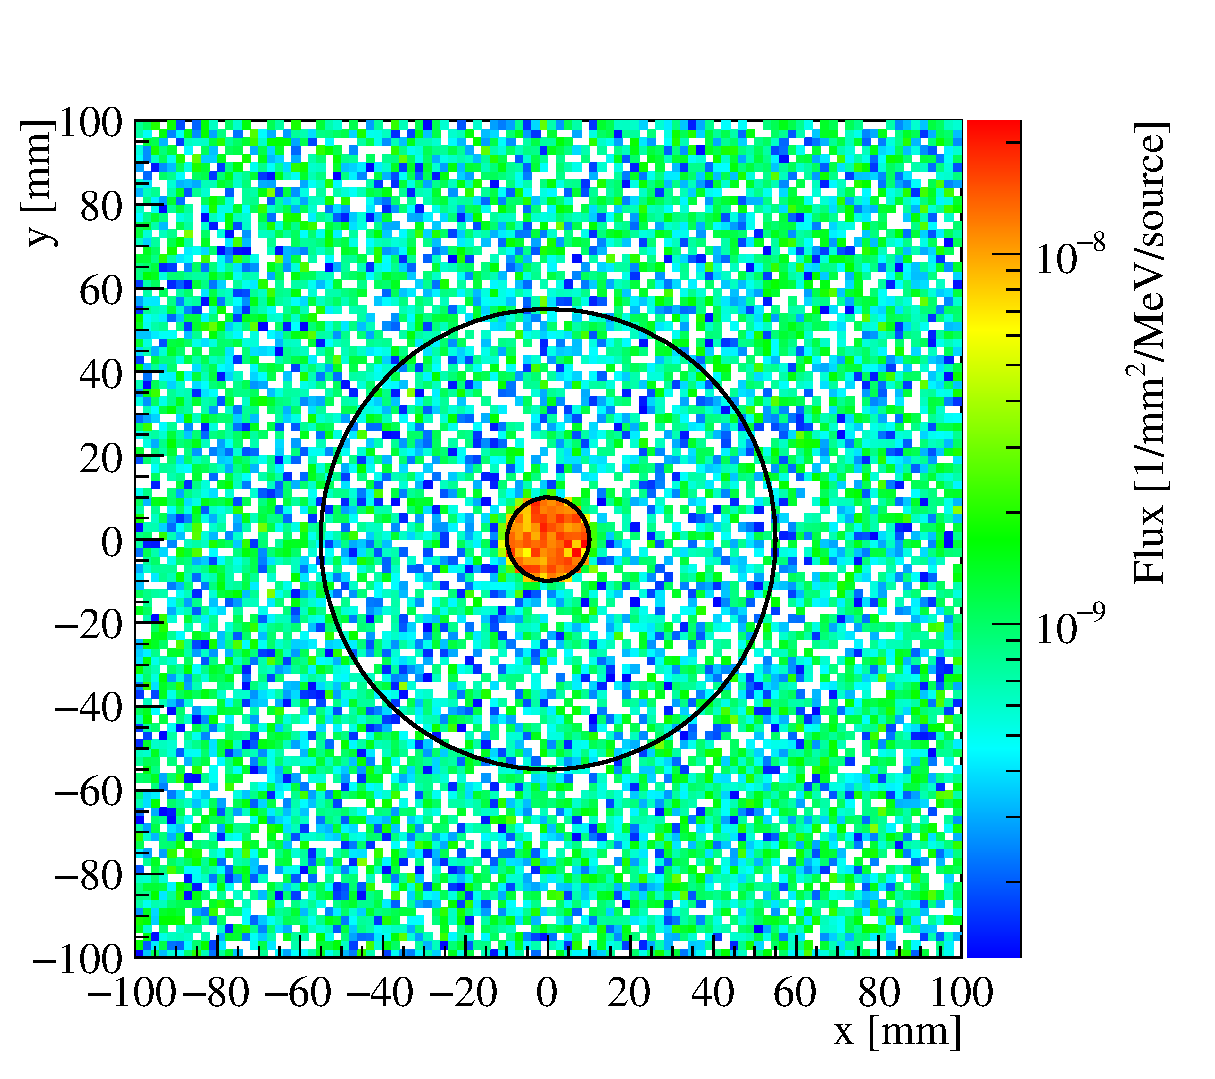
\includegraphics[clip, width=0.7\columnwidth]{cross_xy_f_w_l.eps}
    \caption{ポリエチレンの場合.}
  \end{subfigure}
  \begin{subfigure}{\columnwidth}
    \centering
    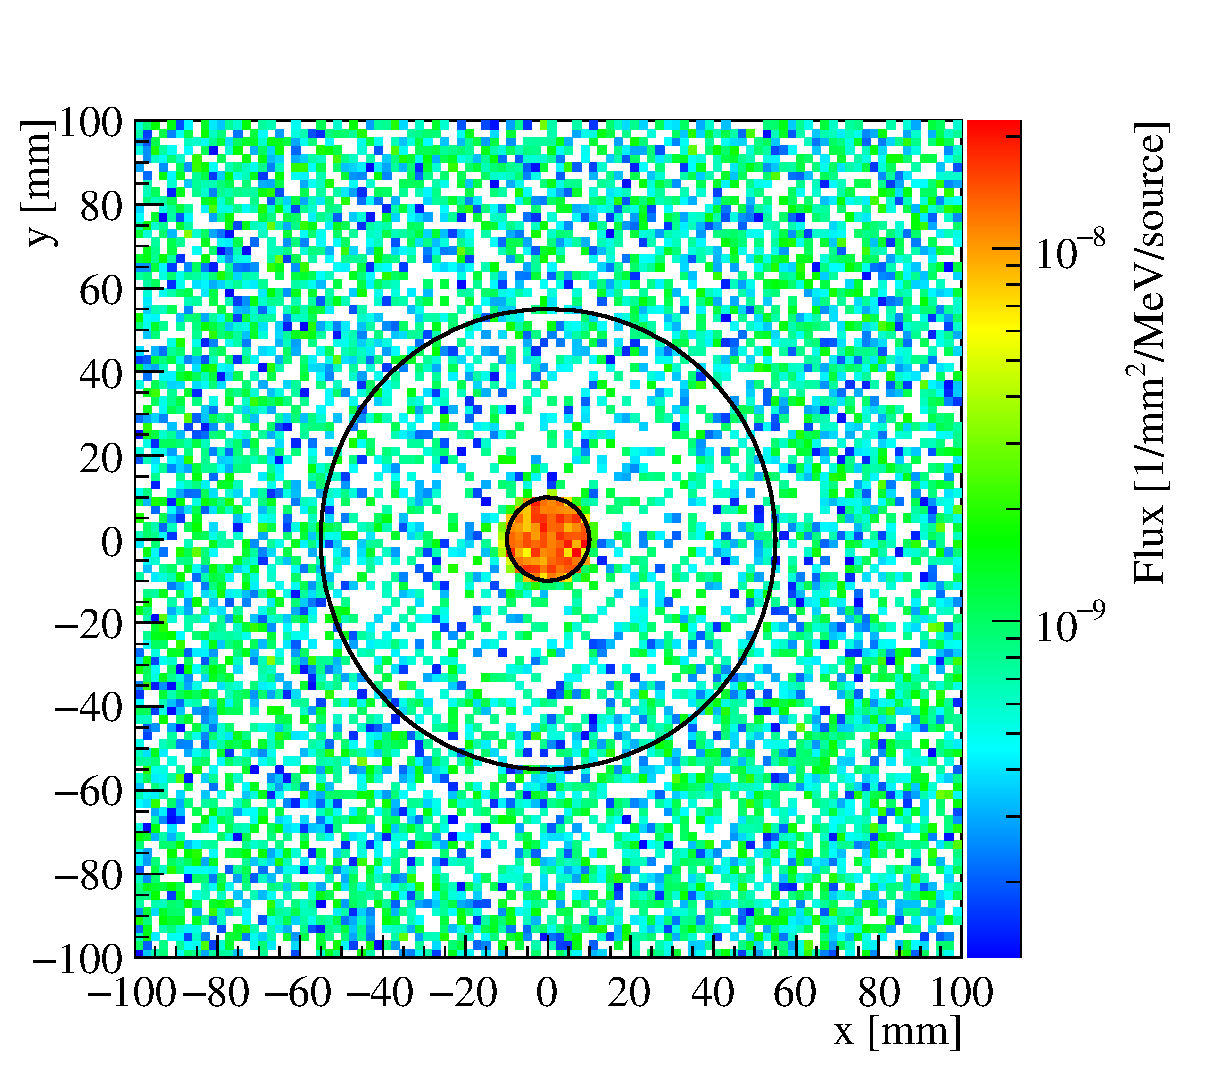
\includegraphics[clip, width=0.7\columnwidth]{cross_xy_f_w_B_w_l.eps}
    \caption{ホウ素入りポリエチレンの場合.}
  \end{subfigure}
  \caption[コリメータ通過後の中性子の位置分布.]
          {コリメータ通過後の中性子の位置分布.2つの円はコリメータの穴と外縁を表す.}
  \label{collimator_xy_pos}
\end{figure}
\begin{figure}
  \begin{subfigure}{\columnwidth}
    \centering
    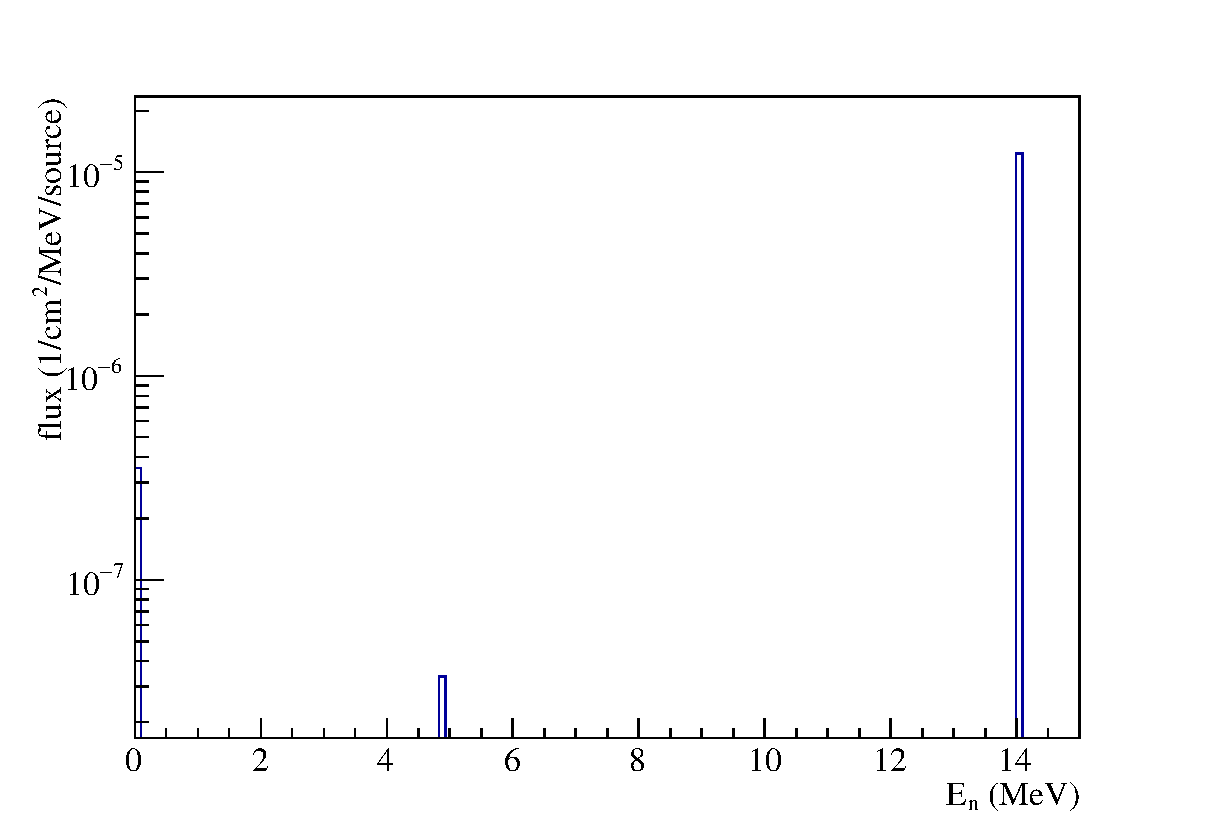
\includegraphics[clip, width=0.8\columnwidth]{cross_eng_f.eps}
    \caption{ポリエチレンコリメータの場合.}
    \label{fig::neutron_energy_dist}
  \end{subfigure}
  \begin{subfigure}{\columnwidth}
    \centering
    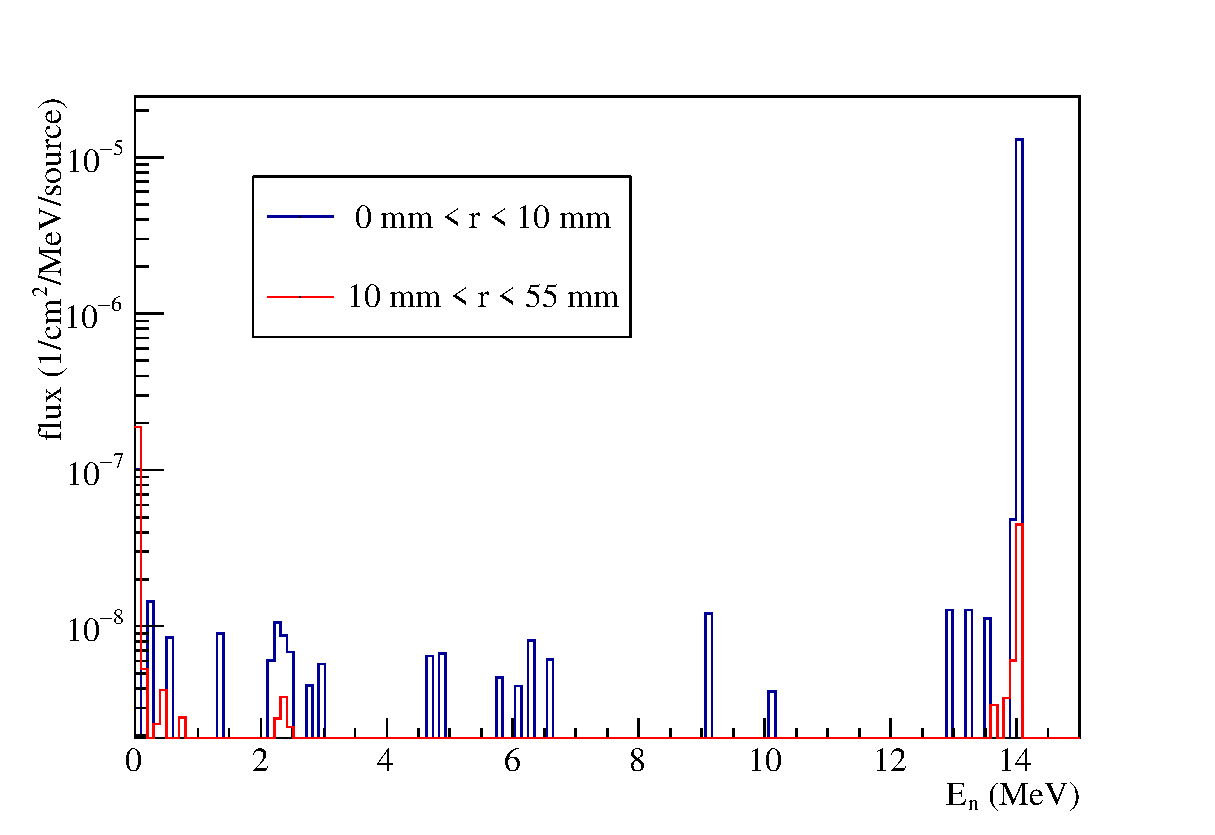
\includegraphics[clip, width=0.8\columnwidth]{cross_eng_f_w_B.eps}
    \caption{ホウ素入りポリエチレンコリメータの場合.}
    \label{fig::neutron_energy_dist_w_B}
  \end{subfigure}
  \caption[中性子のエネルギー分布.]
          {中性子のエネルギー分布.\SIrange{0}{10}{\milli\metre}はコリメータの穴の部分,
          \SIrange{10}{55}{\milli\metre}はコリメータの部分である.}
  \label{fig::neutron_energy}
\end{figure}

ポリエチレンとホウ素入りポリエチレンでは同程度にコリメートできているので,
本実験ではコストの面からポリエチレンを用いたコリメータを採用した.
実際に作成したコリメータを図\ref{pic::collimator}に示す.
このコリメータは半径\SI{53}{\milli\metre},高さ\SI{100}{\milli\metre}の円柱の中心に
半径\SI{10}{\milli\metre}の穴を開けた構造になっている.
壁の厚さが\SI{1000}{\milli\metre}であるため,
このコリメータ10 個を中性子の取り出し穴に挿入する.
\begin{figure}
  \centering
  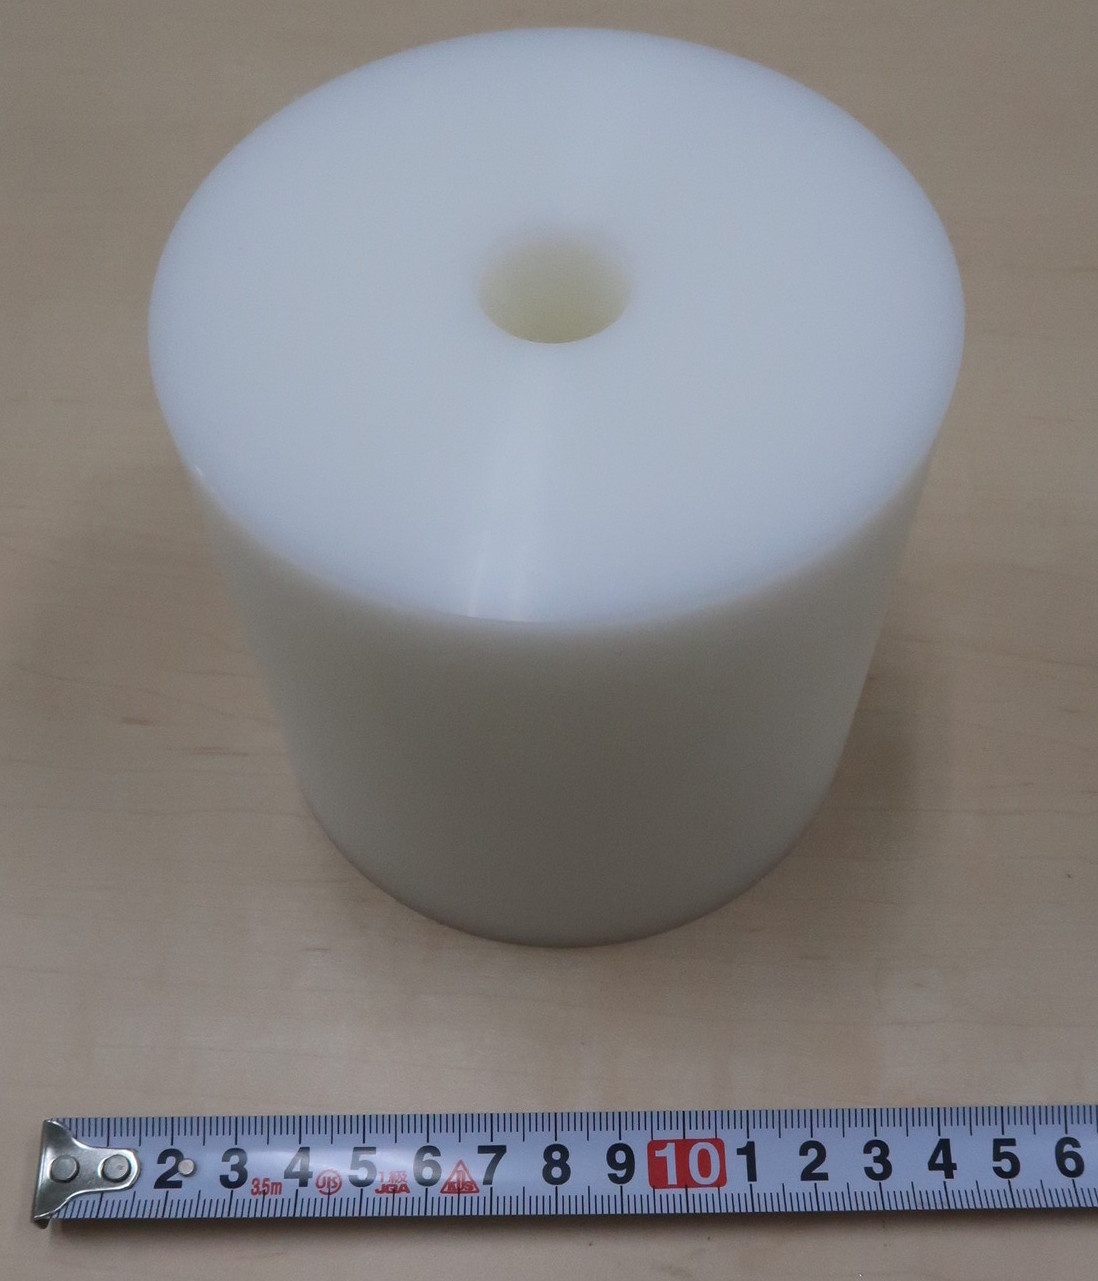
\includegraphics[clip, width=0.8\columnwidth]{IMG_2755_clpd.jpg}
  \caption[ポリエチレンで作成したコリメータ.]
          {ポリエチレンで作成したコリメータ.
            半径\SI{53}{\milli\metre},長さ\SI{100}{\milli\metre}の円柱の中央に,
          半径\SI{1}{\milli\metre}の穴が開いている.}
  \label{pic::collimator}
\end{figure}

\subsection{中性子の収量}
PHITS による計算では\SIrange{0}{10}{\milli\metre}の範囲の
\SIrange{13.9}{14.1}{\mega\electronvolt}の中性子が通過してくる割合は
\SI{8.14e-4}{\percent}となる.
%\SI{4.07e-5}{\per\mega\electronvolt\per source}となる.
OKTAVIAN のDCビームラインで生成される中性子が\SI{5e9}{\per\second}であるとすると,
コリメータを通過してくる\SI{14}{\mega\electronvolt}中性子の量は\SI{4.07e4}{\per\second}となる.

\section{検出効率の散乱位置依存性と散乱角依存性}
\subsection{14~MeV 中性子を用いたとき}
\SI{10}{\milli\metre}のコリメータを用いたときの検出効率は\SI{48.2}{\percent}であった.
検出効率は散乱点,散乱角度に依存していると予想される.
検出効率の散乱点の$z$座標依存性を図\ref{fig::detection_efficiency_beam_axis}に,
${}^{12}\mathrm{C}$の重心系での散乱角 ($\theta_{\text{c.m.}}$) 依存性を図\ref{fig::detection_efficiency_theta_cm}に示す.
%$\theta_{\text{c.m.}}$は入射中性子の運動方向に対する${}^{12}\mathrm{C}$の極角である.
図\ref{fig::detection_efficiency_beam_axis}から分かるように,
$z$座標が小さいまたは大きい場所で反応が起きた場合に,
崩壊してできた$\alpha$粒子が有感領域から出やすくなるため検出効率が低下している.
また,図\ref{fig::detection_efficiency_theta_cm}から分かるように,
$\theta_{\text{c.m.}}$が小さいところで検出効率が低下している.
これは,$\theta_{\text{c.m.}}$が大きいところでは後方散乱となり中性子から多くのエネルギーを受け取り,
崩壊した$\alpha$粒子が全体的に$z$軸正の方向にブーストされることで有感領域から出ていきやすくなるためである.
\begin{figure}
  \centering
  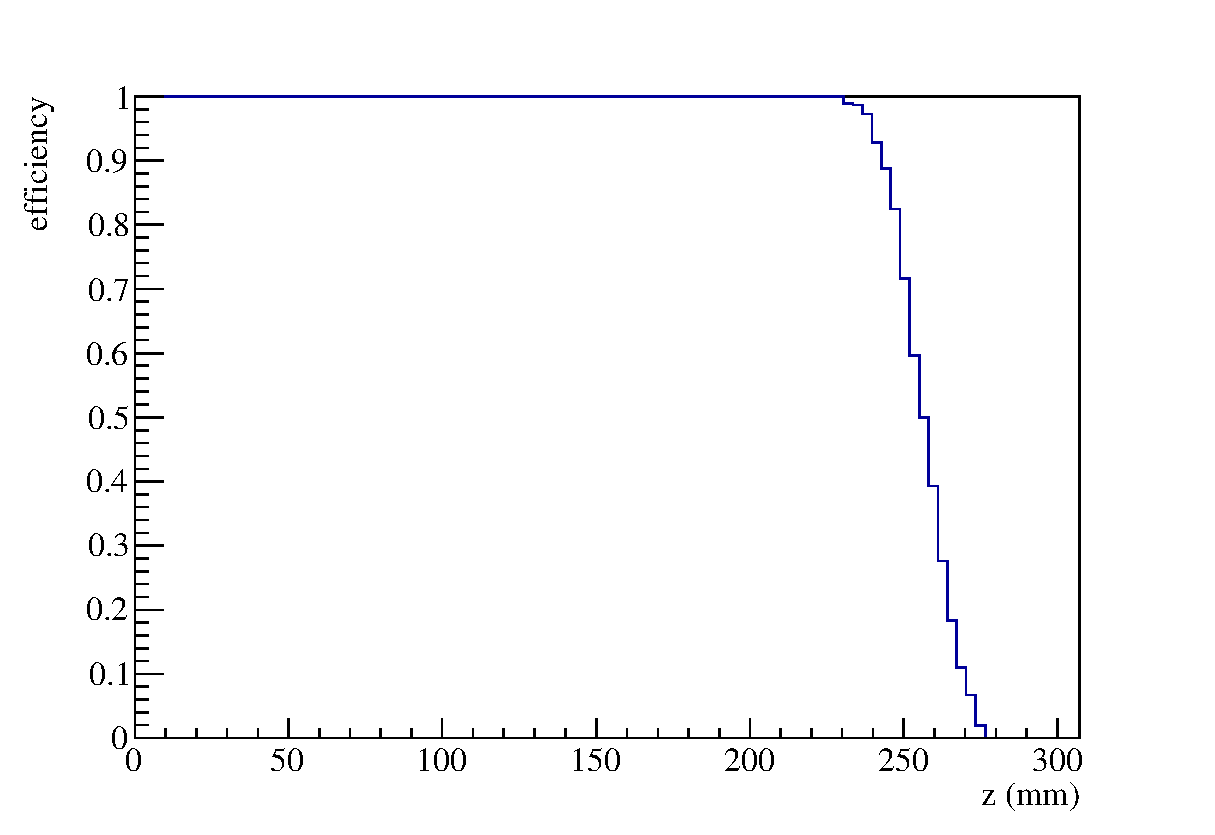
\includegraphics[clip, width=0.8\columnwidth]{detection_efficiency_beam_axis.eps}
  \caption{検出効率の散乱点の$z$座標依存性.}
  \label{fig::detection_efficiency_beam_axis}
\end{figure}
\begin{figure}
  \centering
  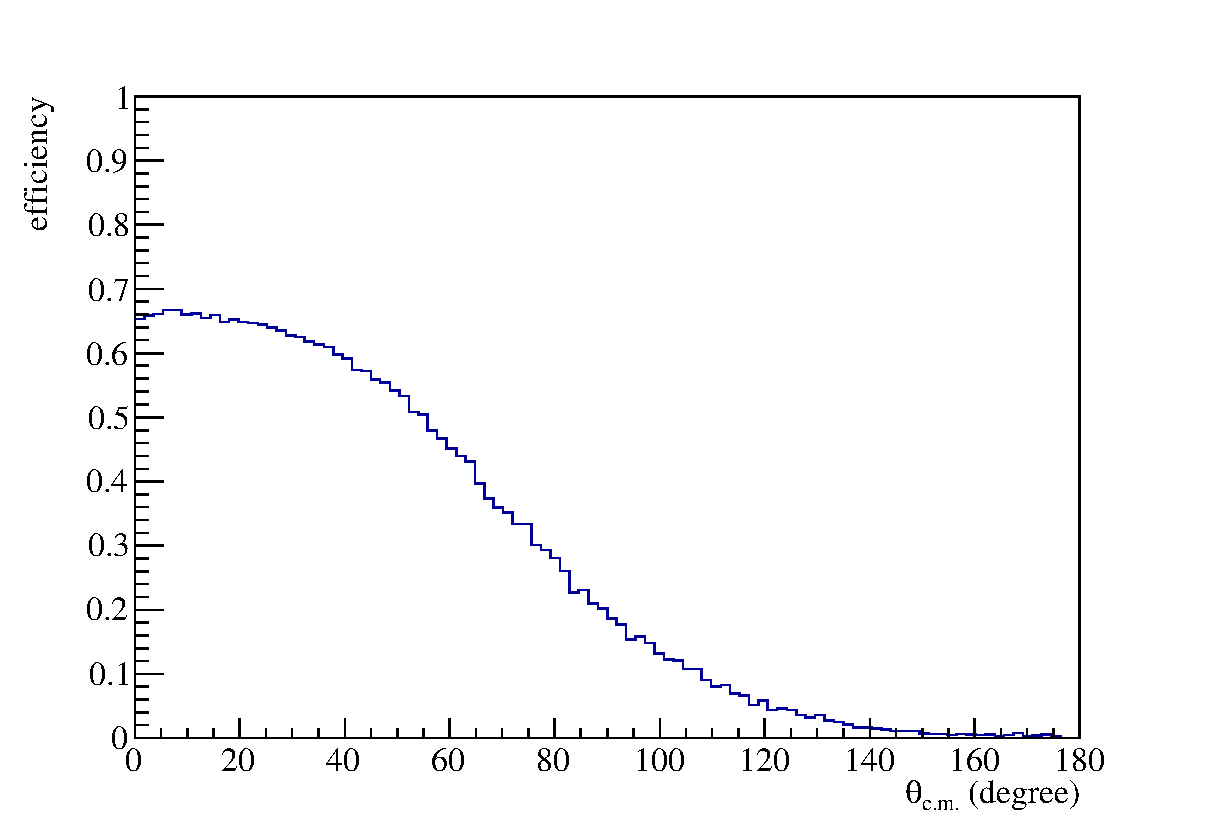
\includegraphics[clip, width=0.8\columnwidth]{detection_efficiency_theta_cm.eps}
  \caption{検出効率の重心系での散乱角依存性.}
  \label{fig::detection_efficiency_theta_cm}
\end{figure}
%\begin{figure}
%  \centering
%  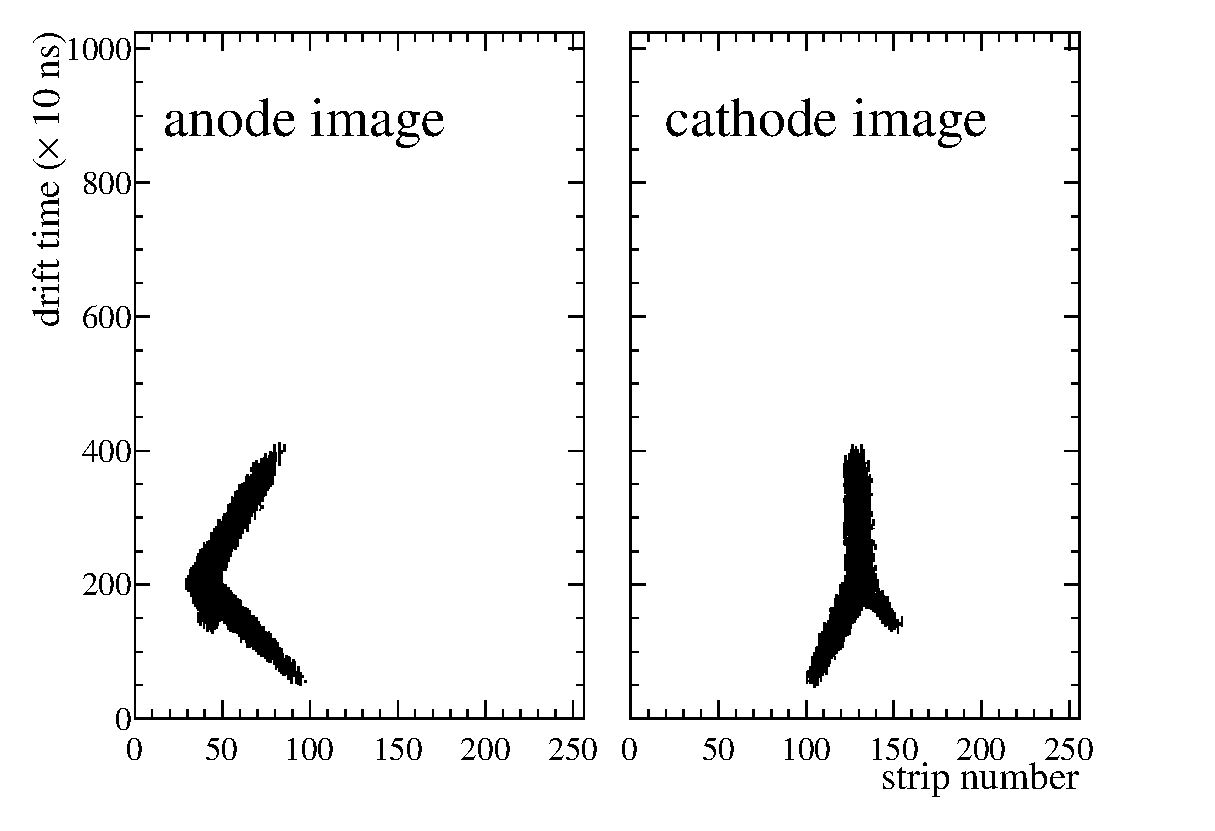
\includegraphics[clip, width=0.8\columnwidth]{10024_12.eps}
%  \caption{$\theta$が小さいときのイベント.}
%  \label{fig::back_sca_event}
%\end{figure}
%\begin{figure}
%  \centering
%  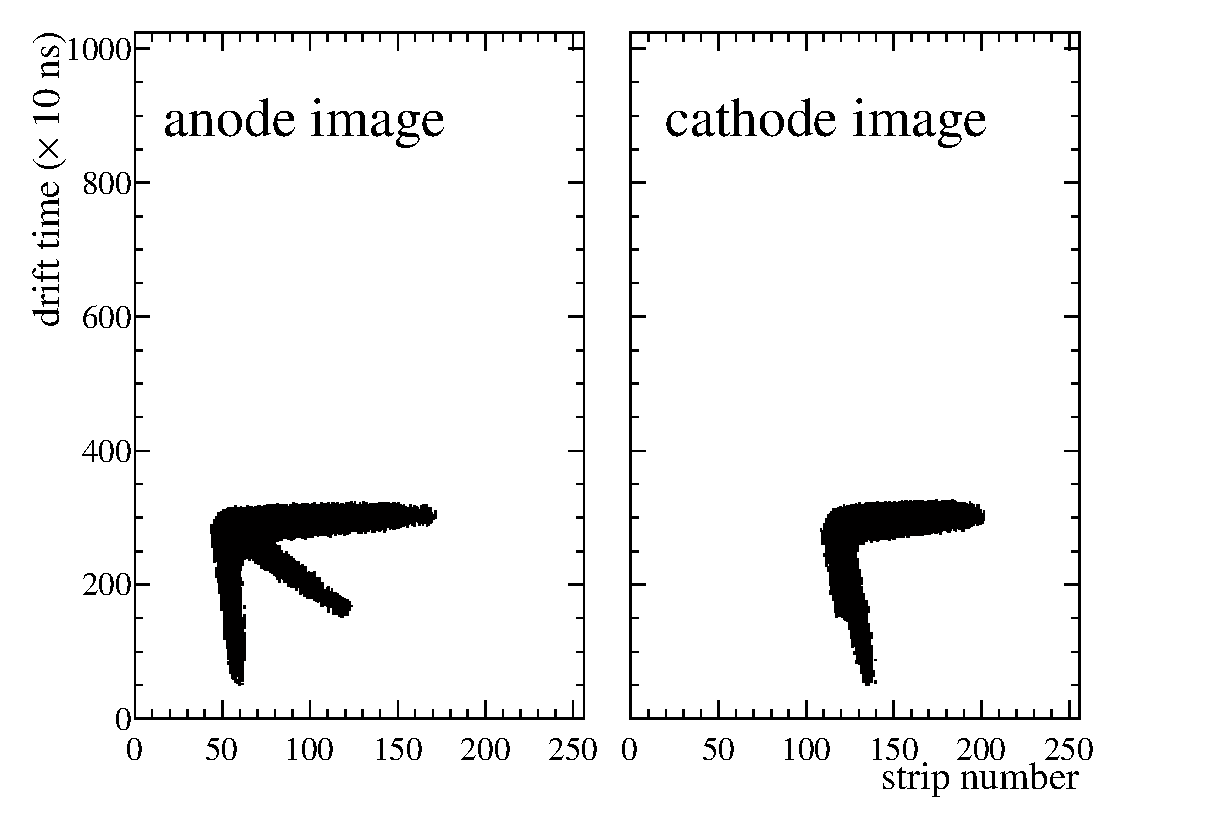
\includegraphics[clip, width=0.8\columnwidth]{10024_74.eps}
%  \caption{$\theta$が大きいときのイベント.}
%  \label{fig::forward_sca_event}
%\end{figure}

\subsection{8.5~MeV 中性子を用いたとき}
${}^{12}\mathrm{C}$を$0_2^+$状態に励起させることができる中性子エネルギーの閾値近傍の断面積が重要となる.
そこで,\SI{8.5}{\mega\electronvolt}の中性子を用いた測定を考える.
テスト実験と同様に\SI{50}{\hecto\pascal}の\isoButaneHydro を用いたMAIKo TPC の運用を仮定する.
また,同じ中性子コリメータを用いるとする.
すると,検出効率は\SI{51.6}{\percent}となる.
微分断面積の角度分布は\SI{14}{\mega\electronvolt}の中性子と${}^{12}\mathrm{C}$の散乱と同じであると仮定した.
検出効率の散乱点の$z$座標依存性を図\ref{fig::detection_efficiency_beam_axis_low}に,
${}^{12}\mathrm{C}$の重心系での散乱角 ($\theta_{\text{c.m.}}$) 依存性を
図\ref{fig::detection_efficiency_theta_cm_low}に示す.
図\ref{fig::detection_efficiency_beam_axis}と比較して図\ref{fig::detection_efficiency_beam_axis_low}は,
\SI{50}{\milli\metre}よりも大きいところで検出効率が小さく,小さいところでは検出効率が大きくなっていることが分かる.
これは,前方散乱に置いて\SI{14}{\mega\electronvolt}中性子のほうが\SI{8.5}{\mega\electronvolt}中性子のほうが
エネルギーの移行が小さいためである.
例えば,$\theta_{\text{c.m.}} = \ang{0}$のとき,
\SI{14}{\mega\electronvolt}中性子と散乱した${}^{12}\mathrm{C}(0_2^+)$の
エネルギーは\SI{0.133}{\mega\electronvolt}であるのに対し,
\SI{8.5}{\mega\electronvolt}中性子と散乱した${}^{12}\mathrm{C}(0_2^+)$のエネルギーは
\SI{0.436}{\mega\electronvolt}である.
すると,3つの$\alpha$粒子が前方にブーストされるため,有感領域の下流側で散乱すると検出率が低下すると考えられる.
その一方,\SI{8.5}{\mega\electronvolt}中性子では,後方散乱したときと前方散乱したときとで${}^{12}\mathrm{C}(0_2^+)$の
エネルギーがあまり変わらないので,横方向に大きく散乱されることがなくなる.
そのため,有感領域の上流側で散乱が起きた場合には大きな検出効率となる.
また,散乱角度によらずに${}^{12}\mathrm{C}(0_2^+)$のエネルギーが変わらないので,
図\ref{fig::detection_efficiency_theta_cm_low}のように検出効率が散乱角度にあまり依存しない.
\begin{figure}
  \centering
  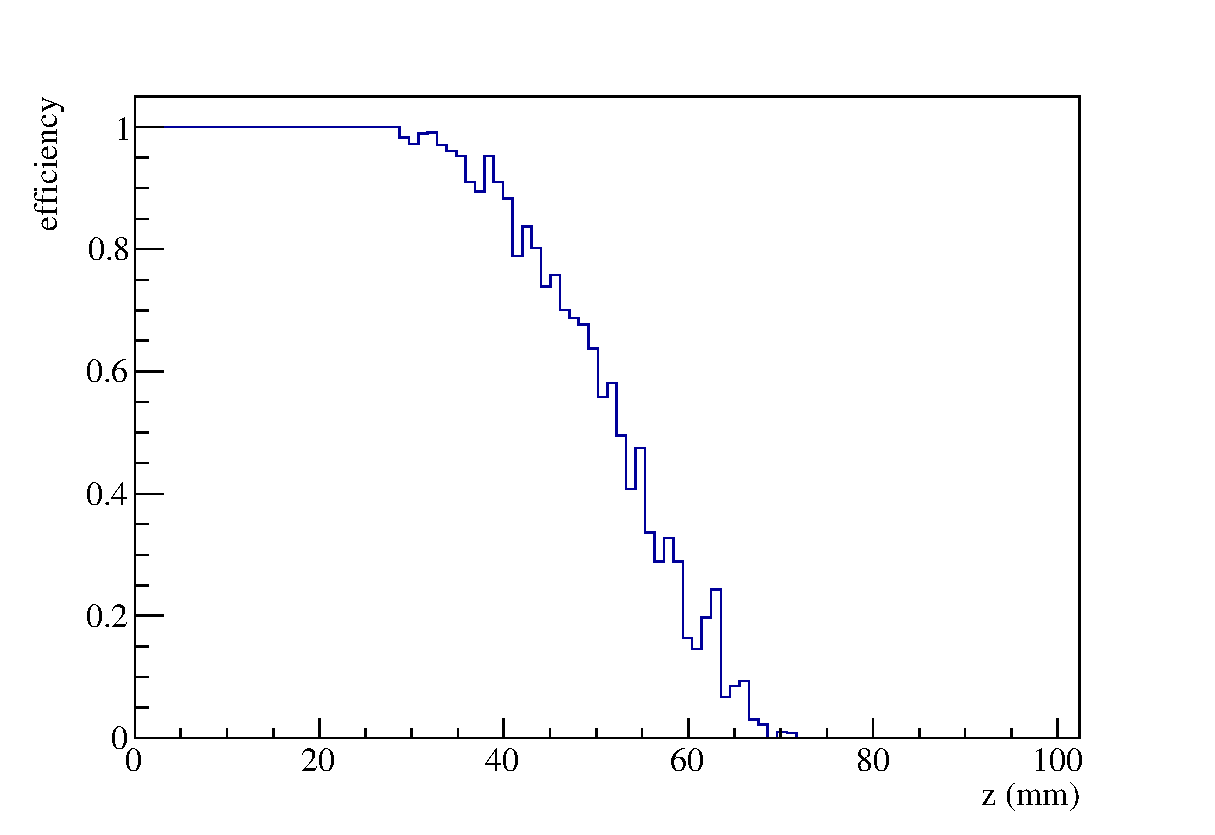
\includegraphics[clip, width=0.8\columnwidth]{detection_efficiency_beam_axis_85.eps}
  \caption{\SI{8.5}{\mega\electronvolt}の中性子を用いたときの検出効率の散乱点の$z$軸依存性.}
  \label{fig::detection_efficiency_beam_axis_low}
\end{figure}
\begin{figure}
  \centering
  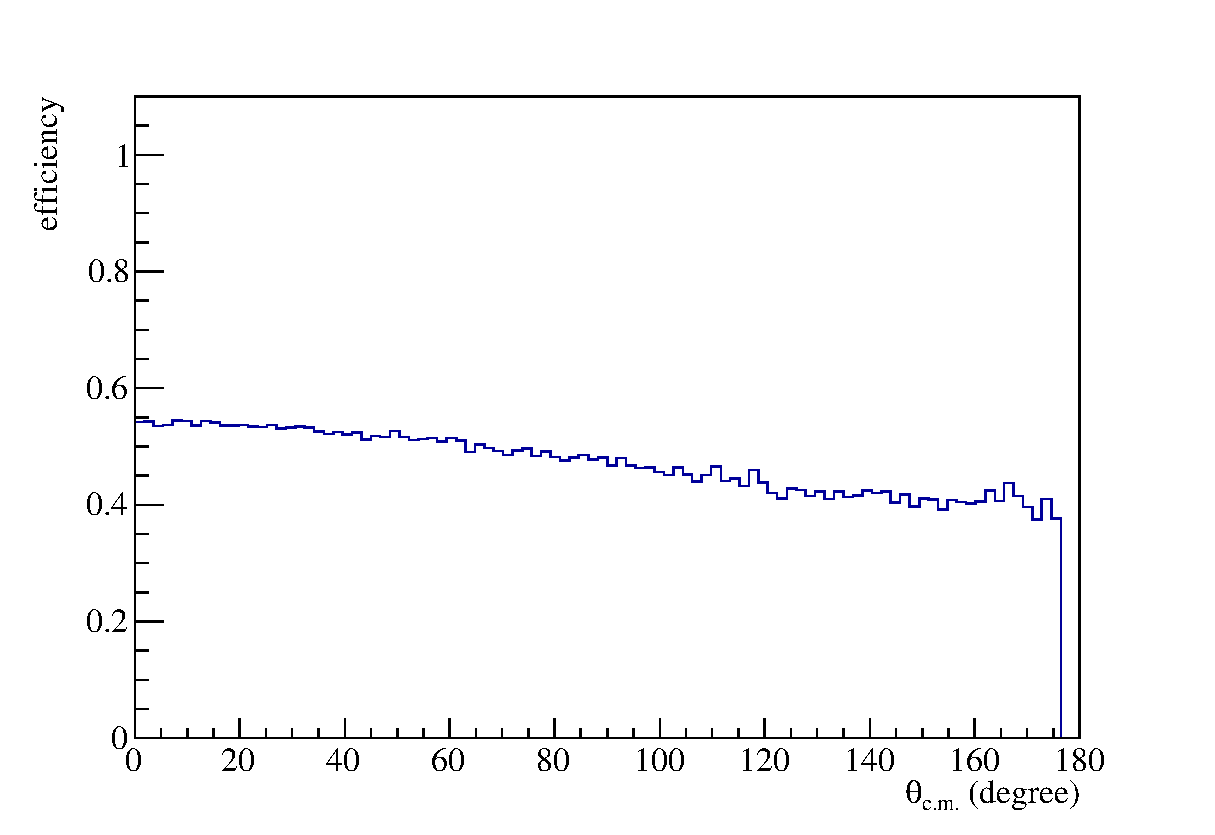
\includegraphics[clip, width=0.8\columnwidth]{detection_efficiency_theta_cm_85.eps}
  \caption{\SI{8.5}{\mega\electronvolt}の中性子を用いたときの検出効率の散乱角依存性.}
  \label{fig::detection_efficiency_theta_cm_low}
\end{figure}

\SI{8.5}{\mega\electronvolt}の中性子を用いたときのシミュレーションから解析効率も評価した.
図\ref{fig::three_alpha_low_En}にシミュレーションで得られた3$\alpha$イベントの一例を示す.
\SI{14}{\mega\electronvolt}のときと同様にeye-scan によって解析を行った.
eye-scan で決定したトラックの本数を表\ref{tab::eye-scan_low}に示す.
\SI{14}{\mega\electronvolt}のときと同様に高い割合で3つのトラックを識別できていることが分かる.
図\ref{fig::ExC_low}にeye-scan で決定した${}^{12}\mathrm{C}^{*}$の励起エネルギーを示す.
励起エネルギー分布の平均は\SI{7.68}{\mega\electronvolt},標準偏差は\SI{17.0}{\kilo\electronvolt}であり,
励起エネルギーも良く再構成されていることが分かる.
本研究で考えている実験条件では,中性子のエネルギーに関わらず測定を行うことができることが分かる.
\begin{figure}
  \centering
  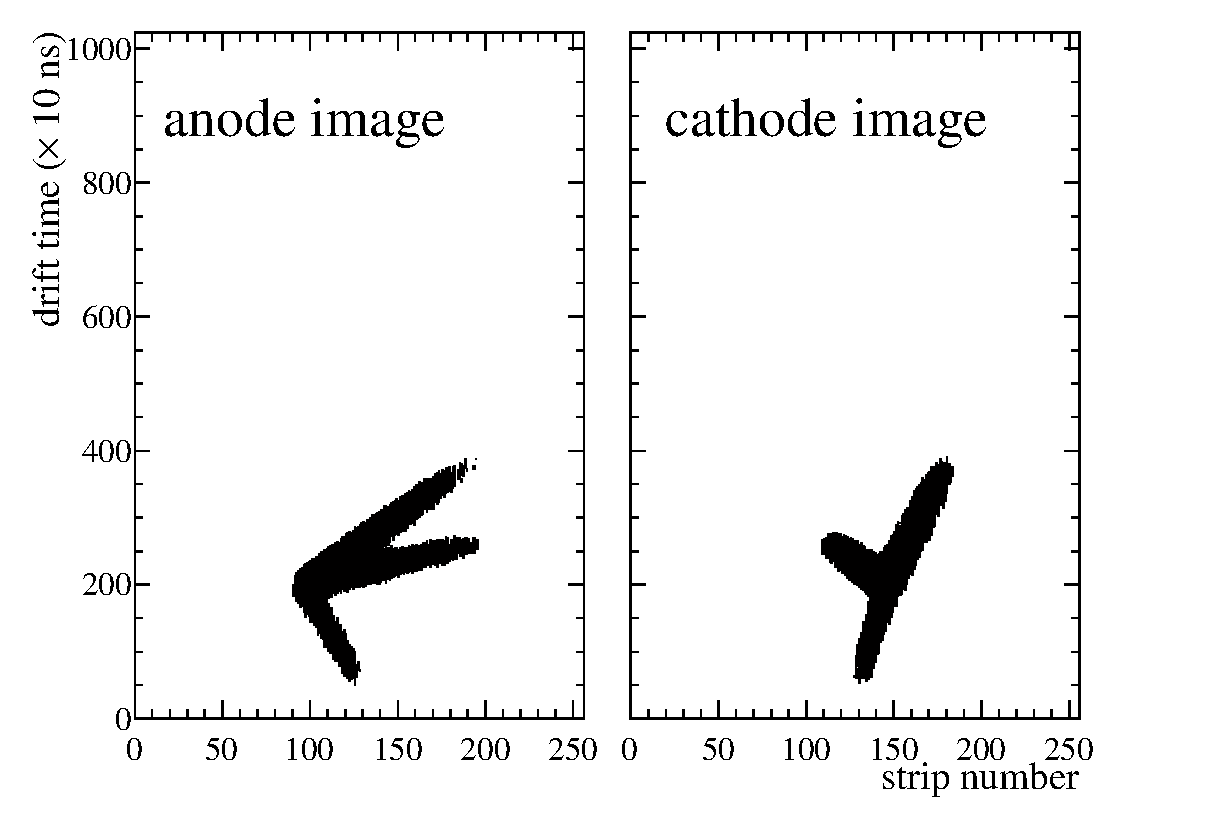
\includegraphics[clip, width=0.8\columnwidth]{10040_2.eps}
  \caption{\SI{8.5}{\mega\electronvolt}の中性子を用いたときのシミュレーショントラックの一例.}
  \label{fig::three_alpha_low_En}
\end{figure}
\begin{table}
  \caption{eye-scan によって決定したトラックの本数.}
  \label{tab::eye-scan_low}
  \centering
  \begin{tabular}{cc}
    \toprule
    トラックの本数 & イベント数 \\
    \midrule
    3 & 93 \\
    2 & 7 \\
    1 & 0 \\
    \bottomrule
  \end{tabular}
\end{table}
\begin{figure}
  \centering
  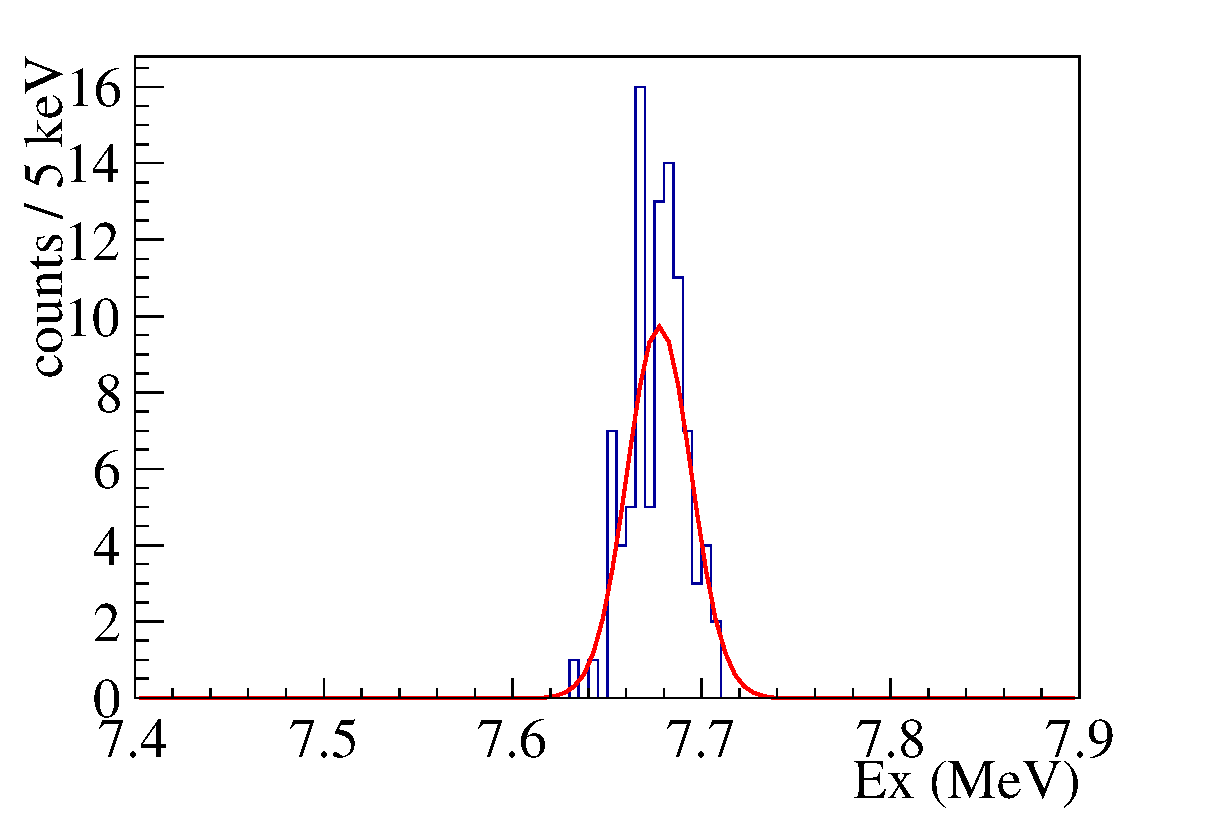
\includegraphics[clip, width=0.8\columnwidth]{ExC_10040_fit.eps}
  \caption{eye-scan によって再構成した励起エネルギー.}
  \label{fig::ExC_low}
\end{figure}

\section{期待される収量}
Ref.~\cite{takahashietal,kondoetal}によると${}^{12}\mathrm{C}(\mathrm{n},\mathrm{n}'){}^{12}\mathrm{C}(0_{2}^{+})$の
断面積 ($\sigma$) は\SI{8.36}{\milli\barn}である.
OKTAVIAN で現在得られるビーム量は最大で$4\pi$に\SI{5e9}{\per\second}である.
この時,半径\SI{10}{\milli\metre}のコリメータからは,$N_{\text{b}}=$\SI{1.95e4}{\per\second}の中性子が得られる.
検出効率 ($\varepsilon_{\text{det.}}$) が\SI{48.2}{\percent},
解析効率 ($\varepsilon_{\text{ana.}}$) が\SI{87}{\percent}である.
\SI{100}{\hecto\pascal}の\isoButaneHydro における有感領域中の${}^{12}\mathrm{C}$の
面密度 ($N_{\text{t}}$) は\SI{1.01e17}{\per\square\milli\metre}である.
%\SI{9.904e-3}{\per\cubic\milli\metre}%\rho = 2.3846e-5\gram\per\cubic\cm
この時,${}^{12}\mathrm{C}(\mathrm{n},\mathrm{n}'){}^{12}\mathrm{C}(0_{2}^{+})$反応の収量は
\begin{align}
  Y &= N_{\text{t}}\times N_{\text{b}}\times \sigma \times\varepsilon_{\text{det}}\times\varepsilon_{\text{ana}} \notag\\
  &= \SI{1.01e17}{\per\square\milli\metre}\times\SI{1.95e4}{\per\second}\times\SI{8.36}{\milli\barn}
  \times\SI{48.2}{\percent}\times\SI{87}{\percent} \notag\\
  &= \SI{6.90e-4}{\per\second}
\end{align}
となる.
24時間の測定で,収量が59.6~events と期待される.

\end{document}
